\chapter{Testing and deterministic verification}

\section{Engineering principles}

Verification must not depend on the model asserting correctness. Unit tests isolate functions; integration tests check boundaries; contract tests check compatibility; end-to-end tests check real workflows. Property tests explore input classes and mutation tests reveal weak assertions. Static analysis, type checking, linting, architecture checks and security scans cover distinct failure modes. Existing passing tests do not establish complete specification coverage.

\section{Implementation approach}

Run trusted tests against the candidate, using a verifier that cannot be modified by the worker. Capture exit code, tool version, commit SHA and artifact digest. Fail the gate on missing reports, skipped mandatory tests or nonzero status. Permit a bounded repair attempt with sanitized diagnostics, then escalate. Include regression and negative tests for invalid inputs and security invariants.

\section{Verification and limitations}

Never accept a patch that removes a failing test or changes the expected outcome without a requirement change and approval. The packaged local verifier checks a toy application and file scope; production must isolate execution and protect the entire trusted test suite.

Figure~\ref{fig:d22} illustrates the conceptual flow from Patch to Repair or stop. The edges describe the proposed integration or control relationship, not undocumented internal calls.

\begin{figure}[htbp]\centering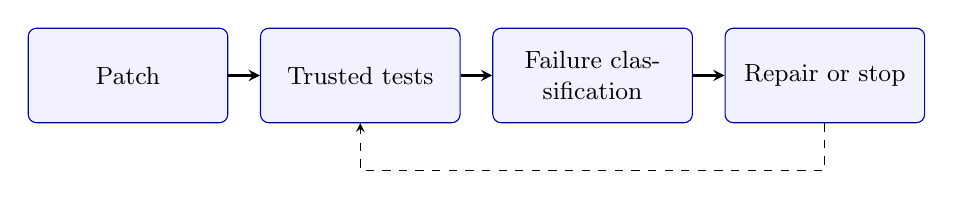
\begin{tikzpicture}[nodebox/.style={draw=blue!60!black,fill=blue!5,rounded corners=3pt,minimum height=12mm,text width=23mm,align=center,font=\small},>=stealth]
\node[nodebox] (n0) at (0.00,0.00) {Patch};
\node[nodebox] (n1) at (2.95,0.00) {Trusted tests};
\node[nodebox] (n2) at (5.90,0.00) {Failure classification};
\node[nodebox] (n3) at (8.85,0.00) {Repair or stop};
\draw[->,thick] (n0.east) -- (n1.west);
\draw[->,thick] (n1.east) -- (n2.west);
\draw[->,thick] (n2.east) -- (n3.west);
\draw[->,dashed] (n3.south) -- ++(0,-.6) -| (n1.south);
\end{tikzpicture}
\caption{Deterministic verification loop (conceptual view).}\label{fig:d22}\end{figure}

\section{Chapter conclusion}

Apply the stated verification criteria before expanding the scope of this workflow. Record deviations, evidence and unresolved risks in the task record.
